\section{Customer content and model privacy}\label{confidential-customer-inference}

\subsection{Public \textit{A} and private \textit{B} execution}\label{customer-execution-modes}

The service must keep customer prompts, responses, reference writing, and
derived representations inaccessible to miners. Usage metadata, including
timing, token counts, and cost, may be visible. Private \textit{B} weights must
also be inaccessible for download by the general public. Cloudflare and
SlopNinja are trusted with content; either may technically access hosted model
weights. The proposal therefore offers no cryptographic confidentiality from
those operators, no independent customer key release into attested hardware,
and no TEE execution claim.

For \textit{A}, SlopNinja runs a selected published artifact in its own runtime.
The model contributor receives neither customer traffic nor an account with
access to its storage. Artifacts submitted to a cohort are private evaluation
material until that cohort's scoring starts. Miners upload them straight to the
coordinator's private R2 admission storage through presigned URLs, protected in
transit by TLS and at rest by the bucket's access controls rather than an added
encryption layer, and they are never served to customers before publication. Customers may instead download published artifacts and
run them locally, subject to their dependencies and execution contract. Such a
run creates no hosted job, customer charge, or inference credit.

The proposed later \textit{B} path gives a miner control of its private LoRA
adapter and Cloudflare billing account while SlopNinja controls each request.
The miner privately delegates an account-scoped Workers AI credential and
registers the account, base model, and adapter UUID. SlopNinja stores the
credential and constructs the direct Workers AI request itself. The customer
receives neither that credential nor an adapter asset URL. The numeric ranker
is uploaded separately to private SlopNinja storage and loaded only by our
runtime. Neither account ownership nor a private adapter gives the miner a
place in the customer's request or response path.

Tests found that the Workers AI Read grant also permits adapter-asset download.
The design accepts that SlopNinja can technically read those weights. A
dedicated serving account can limit the other assets exposed by this grant.
Public asset denial, including attempts by an unrelated authenticated account,
must be qualified before private serving. Keeping weights private does not
prevent behavioral imitation or extraction through purchased outputs.

\begin{figure}[htbp]
\centering
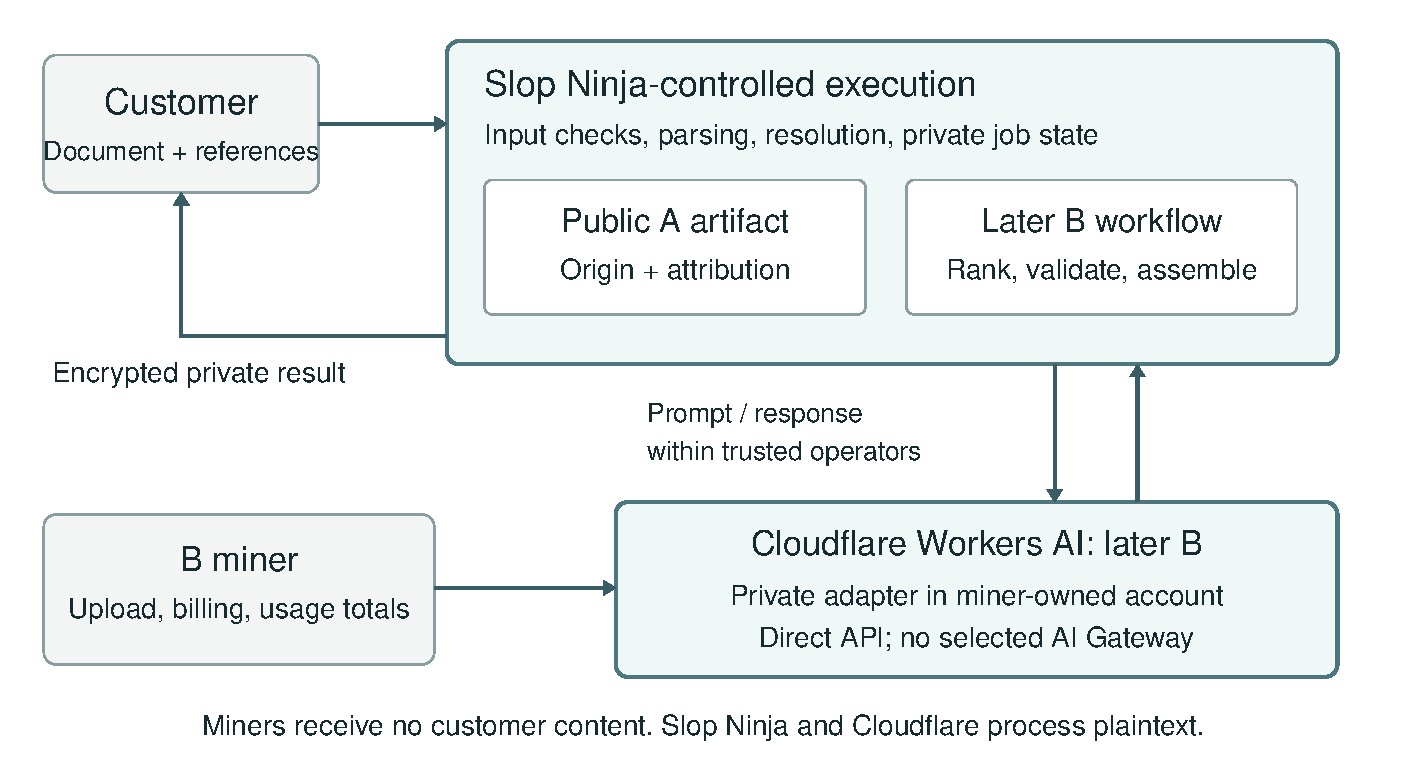
\includegraphics[width=\linewidth]{figures/private-inference.pdf}
\caption{Proposed customer execution paths. Public \textit{A} runs under SlopNinja's
control. Later \textit{B} uses a miner's billed Cloudflare account through direct
operator requests. Content isolation from that account's owner requires the
qualification described below; the diagram states the intended boundary.}
\end{figure}

\subsection{Direct serving and content logging}

The runtime sends synchronous calls to Cloudflare's direct Workers AI endpoint
for the enrolled account and base model, selecting the registered adapter UUID.
It omits AI Gateway selection, including the \texttt{cf-aig-gateway-id} header,
and accepts no miner endpoint, Worker, callback, or logging destination. It
forwards no caller-supplied routing headers and follows no redirects to miner
destinations. Provider-side batch jobs and stored conversations are excluded
because they may create additional owner-readable result surfaces. Cloudflare's
published data policy is an accepted provider assumption~\cite{cfdatausage};
the direct REST and gateway interfaces define different request
paths~\cite{cfdirectai,cfaigateway}.

The reported owner-session inspection on October 22, 2026 found aggregate usage
and no prompt or response text for the synthetic direct requests on the inspected
dashboard, audit, and observability surfaces~\cite{cfownerinspection}. The cited
record distinguishes that operator-supplied browser report from the direct API
checks, which also exposed per-request usage metadata. No AI Gateway existed
during those requests. This observation does not establish that an account
owner can never enable content capture. Before paid \textit{B} activation, run a controlled
comparison with gateway logging enabled: a routed positive control must appear,
and a direct request without gateway selection must remain unavailable. Examine
owner controls that could capture that direct request. Provider changes require
renewed qualification; absence from the surfaces inspected so far is limited
evidence, not a universal privacy proof.

Returned identity associates a response with the selected adapter under
Cloudflare's API behavior. It does not attest immutable weights or an unchanged
hosted base model. Enrollment checks private asset digests, updates receive
fresh version registrations and adapter UUIDs, and detected drift suspends
service. Periodic checks cannot exclude a change-and-restore race. Receipts state
the observed identity and enrolled digests without asserting a historical
measurement that the provider does not supply.

\subsection{Storage, isolation, and recovery}\label{assignment-recovery-and-the-privacy-boundary}

Customers submit over authenticated encrypted transport to SlopNinja. The
runtime processes plaintext, then encrypts the result to the customer's bound
output key for private retrieval. Private storage uses tenant authorization,
encryption, and declared retention. Operational logs contain identifiers,
usage, transitions, and normalized errors; provider errors must be sanitized
because they can echo a prompt. Content logging is disabled in Workers, traces,
and support tools. Profiles, vectors, intermediate candidates, and, for later
\textit{B}, parse trees and cached resolver outputs receive the same protection
as the original text. \textit{B}'s parsing and ambiguity resolution, including
any LLM resolver, run within the same SlopNinja and Cloudflare trust boundary;
miners receive neither resolver inputs nor outputs.

Each attempt binds its customer, job, assignment generation, model and pipeline
version, output key, and resource limits. State from one customer must not enter
another job. Recovery resumes only authorized durable state; reassignment
cannot silently introduce a new content recipient. A lost key or unavailable
result follows the job's failure and refund terms. Customer retention deadlines
remain in force during an evaluation pause. Preserving an unfinished benchmark
cohort indefinitely grants no authority to retain customer documents indefinitely.

Public receipts omit raw document hashes, filenames, titles, and report URLs.
Validator-accessible R2 inference receipts also exclude prompts, responses,
held-out labels, and parsed vectors. Their certified package and rolling
two-cohort deletion rule appear in Section~\ref{cohort-receipt-retention};
receipt access supplies no right to underlying content or commitment openings.
Content commitments use canonical encoding, a fresh secret salt, and separate
domains and lengths, for example:
\begin{equation}\label{eq:input-commitment}
C=\operatorname{SHA256}\bigl(
\mathrm{domain}\mathbin\Vert\mathrm{context}\mathbin\Vert
\mathrm{salt}\mathbin\Vert\mathrm{length}\mathbin\Vert
\mathrm{payload}\bigr).
\end{equation}
Salts and openings remain private. The context binds the deployment and job;
the output record also binds the customer's key and complete encrypted object's
digest and length. A commitment proves consistency when opened, not execution,
truth, or delivery. Result availability for the quoted retention period remains
an operator service obligation.

Model outputs are untrusted data. The runtime executes no generated tools,
URLs, or callbacks, and enforces schemas, budgets, and size limits. The result
viewer renders inert text without remote images or automatic link previews.
MCP delivery does not authorize commands embedded in a document. These controls
also apply to hostile source text and grammar contributions. An independent
security review before paid \textit{B} launch must test routing, credential
storage, content logging, cross-job isolation, and result access under this
provider-and-operator trust model.

A malicious adapter could encode prompt information in its output length,
exposing bits through owner-visible token counts or billed usage even when
content logging is disabled. Review must test this active channel and assess
fixed-size generation or output-size bucketing at the provider's metering
boundary. Padding the returned result cannot hide counts already metered by
the provider; a maximum output limit alone cannot close the channel. Ordinary
metadata visibility is accepted, but a demonstrated path to recover customer
content blocks paid \textit{B} activation until addressed. Mandatory traffic
padding is not otherwise part of the proposal, and passive metadata inference
remains a stated limit.

\subsection{Customer-directed disclosure}\label{customer-directed-evidence-disclosure}

A dispute gives validators no automatic right to read customer text. A customer
may authorize a separate disclosure naming the recipient, purpose, material,
and validity window. Further recipients require further authorization. Partial
evidence supports only a limited finding and cannot open a commitment to an
entire document. Expiry limits subsequent authorized processing but cannot
erase plaintext already received. Editorial review is advisory unless the
accepted service terms specify a remedy.

External detectors, including Pangram, receive customer content only with
separate authorization and funding. A service's benchmark record is not a live
external-detector result for the customer's document. Customer material enters
training only with separate opt-in; on-chain accounting and validator record
checks create no reuse exception.
